\mychapter{Credential Relationship Binding Nullifier}

\section{Introduction}

In Chapters 2 and 3, we developed a robust foundation for anonymous credentials, evolving from single-issuer Attribute-Based Anonymous Credentials $(\ABC)$ to the Multi-Issuer Multi-Credential ABC $(\MIMCABC)$ system with identity binding security. $\MIMCABC$ enables users to privately prove that credentials from multiple, mutually distrusting issuers belong to the same identity, a significant advance for applications like federated identity proofs or content credentialing. However, real-world identity systems impose additional requirements that $\MIMCABC$ does not fully address: hierarchical structure and sybil resistance for context-specific credentials.

In practice, credentials often form a natural hierarchy, with foundational identities—such as government-issued IDs or passports—serving as Master Credentials, and dependent credentials—like driver’s licenses, professional certificates, or access rights—acting as Context Credentials. This structure enables efficient revocation: invalidating a Master Credential (e.g., upon employment termination) implicitly revokes all dependent Context Credentials, avoiding the need to track and revoke each individually. Furthermore, regulatory frameworks like KYC/AML demand accountability, requiring systems to prevent sybil attacks where users illegitimately obtain multiple credentials for the same context (e.g., multiple driver’s licenses). 

While MIMC-ABC ensures credentials share a single identity, it lacks mechanisms to enforce this hierarchical dependency or prevent sybil attacks in a privacy-preserving manner, as its identity binding operates agnostically across all credentials without distinguishing their roles or contexts. To meet these practical and regulatory needs, we must extend MIMC-ABC with a cryptographic framework that organizes credentials hierarchically and ensures context-specific uniqueness, all while preserving user anonymity and computational efficiency


\subsection{Problem Statement}

We want to improve MIMC-ABC for real-world use. Our goal is a private credential hierarchy with Sybil resistance. A user has a Master Credential with a secret key $\k$. They also have Context Credentials with unique IDs $\ctx$ (e.g., $\mathcal{H}(\text{"DriverLicense"})$). We need a mechanism that:
\begin{enumerate}
    \item Links each Context Credential to the Master Credential. It uses a unique nullifier $\nul$ from committed values $\k$ and $\ctx$ from different commitments.
    \item Prevents sybil attacks. It prevents multiple nullifiers for the same $(k, \ctx)$ pair.
    \item Verifies nullifier correctness in zero-knowledge. It hides $\k$ and $\ctx$.
\end{enumerate}


Our main challenge is:
\begin{center}
\emph{How do we efficiently generate a verifiable nullifier that proves the binding relationship between two separate credentials without leaking any additional information}
\end{center}


\subsection{Background Work}

Past works tackled hierarchy and sybil resistance in credential systems. None fully balances privacy, efficiency, and flexibility. 
\begin{enumerate}
    \item The UTT anonymous payment system ~\cite{tomescu2022utt} is the closest work, using a registration credential (like a Master Credential) and the coins are also credentials using serial numbers (like Context Credentials) where a coin can only be spent once. UTT uses pairings in their pseudorandom function which we benchmark against and show our speedup.

    \item CanDID~\cite{maram2021candid} defines Master and Context Credentials clearly, but has weakened privacy. It uses mappings between credential public keys in a table, breaking unlinkability. It also relies on an MPC-based PRF for sybil resistance. This adds complexity and overhead, unfit for lightweight use.

    \item Other pairing-based systems, like SyRA~\cite{crites_syra_2024} and S3ID~\cite{rabaninejad_attribute-based_2024}, offer private hierarchies. Yet, they suffer from pairing-related efficiency issues and slower zero-knowledge proofs where we use $\Sigma$-protocols, which are the most efficient zero-knowledge proofs.

    \item Standard Verifiable Random Functions  (VRFs)~\cite{hutchison_verifiable_2005} reveal the user’s public key during verification impacting anonymity and furthermore are constructed with bilinear pairings.

\end{enumerate}

Our MIMC-ABC system (Chapter 3) binds identities efficiently and anonymously but without hierarchy and context-specific sybil resistance. We need a solution that keeps MIMC-ABC’s strengths. It must add a light, private way to handle credential hierarchies and sybil resistance.




\subsection{Contributions}

We advance anonymous credential systems by developing a lightweight, pairing-free Verifiable Random Function (VRF) construction optimized for our use-case of hierarchical credential binding and sybil resistance. Our contributions are threefold:

\begin{enumerate}
        \item \textbf{Pairing-Free VRF in Prime-Order Groups:} We adapt the Dodis-Yampolskiy VRF structure for standard prime-order groups by replacing the proof mechnaism and prove our construction retains the security properties - \emph{pseudorandomness, uniqueness, verifiability} - under the $q$-DHI assumption. (We show the efficiency speedup of this change)

        \item \textbf{Novel $\Sigma$-protocol for Multiplicative Inverse:} We develop a novel zero-knowledge proof protocol to prove that two secret exponents (within a commitment) are the multiplicative inverse of each other. We use this protocol to prove the correctness of the $q$-DHI structure used in the Dodis-Yampolskiy VRF, the technique is a new general technique for $\Sigma$-protocols.
        
        \item \textbf{Credential Relationship Binding Nullifier } We combine our efficient Dodis-Yampolskiy VRF for standard prime-order groups with our Novel $\Sigma$-protocol for multiplicative inverse in addition to a $\Sigma$-proof of additive relation between discrete logarithms to compute our nullifier and show it's 33\% faster for evaluation and 60\% faster for verification than previous constructions while retaining security properties.

\end{enumerate}


Levearging our work, we propose the Credential Relationship Binding Nullifier (CRBN) which extends the MIMC-ABC system into a complete identity framework with benefits:

\begin{enumerate}
    \item Cryptographically binds master credentials (containing key $\k$) to context credentials (with context identifiers $\ctx$) via a verifiable nullifier enabling accountability

    \item Enforces sybil resistance for context credentials while retaining privacy by using committed attributes and zero-knowledge proofs

    \item Integrates with the efficient $\Sigma$-protocols used throughout the system
    
\end{enumerate}















\section{Preliminaries}
\subsection{Cryptographic Assumptions}

\begin{definition}[q-DHI Assumption]
Let $\mathbb{G}$ be a cyclic group of prime order $p$ with generator $g$. The $q$-Diffie-Hellman Inversion ($q$-DHI) assumption \cite{mitsunari_new_2002} states that for any PPT adversary $\mathcal{A}$, there exists a negligible function $\negl$ such that:
\[
\Pr\left[ x \sample \Zp^*, \quad \mathcal{A}(g, g^x, g^{x^2}, \ldots, g^{x^q}) = g^{1/x} \right] \leq \negl 
\]
where the probability is taken over the random choice of $x$ and the random coins of $\mathcal{A}$. Informally, no $\PPT$ adversary can distinguish between $g^{1/\alpha}$ from a random group element.
\end{definition}

\begin{remark}
The $q$-DHI assumption is equivalent to the $(q+1)$-generalized Diffie-Hellman assumption (GDH) as shown by Boneh and Boyen \cite{kanade_efficient_2004}. This equivalence provides a solid theoretical foundation for the security of our VRF construction.
\end{remark}


\subsection{Building Blocks}
We use the Pedersen Commitments from chapter 2, committing to a vector of messages $\cm = \CMCom([\id, \ctx, \exp, \k];\usk) = g_1^\id g_2^\ctx g_3^\exp g_4^\k g^\usk$. Pedersen Commitments are hiding, binding, and position-binding which enforces their position in the vector of messages such that the exponent at one position can't be swapped with another position. 

We use the three-move $\Sigma$-protocols \ref{preliminaries-sigmaprotocol} to prove relations of exponents which we represent as $\mathcal{R}_{\mathsf{VRF}} = \left\{(w)(x) \mid x = g^w \right\}$ proving knowledge of secret witness $w$ with public statement $x$. 


\begin{definition}[Verifiable Random Function]
A Verifiable Random Function (VRF) is a tuple of probabilistic polynomial-time algorithms $(\PPT)$ $(\mathsf{VRF.Gen}, \mathsf{VRF.Eval}, \mathsf{VRF.Vfy})$ with an associated message space $\setX$, output space $\setY$ and proof space $\Pi$ defined as:
\begin{itemize}
    \item $\mathsf{VRF.Gen}(1^\lambda) \to (sk, pk)$: Takes a security parameter $\lambda$ and outputs a secret key $sk$ and a public key $pk$.
    
    \item $\mathsf{VRF.Eval}(sk, x) \to (y, \pi)$: On input $x \in \setX$ and secret key $sk$, outputs a value $y \in \setY$ and a proof $\pi \in \Pi$.
    
    \item $\mathsf{VRF.Vfy}(pk, x, y, \pi) \to \{0,1\}$: Using the public key $pk$, verifies that $y$ is the correct output for input $x$ with proof $\pi$, returning 1 if valid, 0 otherwise.
\end{itemize}
    
\end{definition}
A $\VRF$ must satisfy three properties
\begin{itemize}
    \item \textbf{Correctness:} For all $(sk, pk) \gets \mathsf{VRF.Gen}(1^\lambda)$ and all $x \in \setX$:
    \[
    \Pr\left[\begin{aligned}
        (y, \pi) &\gets \mathsf{VRF.Eval}(sk, x) \\
        1 &\gets \mathsf{VRF.Vfy}(pk, x, y, \pi)
    \end{aligned}\right] = 1
    \]

    \item \textbf{Unique Provability:} For any $pk$ (possibly malicious) and $x \in \setX$, no $\PPT$ adversary $\AdvA$ can find two distinct pairs of outputs $(y_0, \pi_0) \neq (y_1, \pi_1)$ such that:
    \[
    \mathsf{VRF.Vfy}(pk, x, y_0, \pi_0) = \mathsf{VRF.Vfy}(pk, x, y_1, \pi_1) = 1
    \]

    \item \textbf{Pseudorandomness:} Informally, this property ensures that without the secret key, the output of the VRF for an unqueried input is indistinguishable from a random value, even when the adversary can see other input-output pairs.
    Formally, For any PPT adversary $\mathcal{A}$, the advantage in the following experiment is negligible:
    \[
    \left|\Pr\left[\begin{array}{l}
        (sk, pk) \gets \mathsf{VRF.Gen}(1^\lambda) \\
        x^* \gets \mathcal{A}^{\mathcal{O}_{\mathsf{VRF.Eval}(sk, \cdot)}}(pk) \\
        (y^*, \pi^*) \gets \mathsf{VRF.Eval}(sk, x^*) \\
        y_0 \gets y^*; \, y_1 \sample \mathcal{Y} \\
        b \sample \{0,1\} \\
        b' \gets \mathcal{A}^{\mathcal{O}_{\mathsf{VRF.Eval}(sk, \cdot)}}(pk, y_b)
    \end{array} : b' = b \wedge x^* \notin \mathcal{Q}\right] - \frac{1}{2}\right| \leq \negl(\lambda)
    \]
    where the oracle $\mathcal{O}_{\mathsf{VRF.Eval}(sk, \cdot)}$ takes input $x \in \mathcal{X}$ (where $x \neq x^*$) and outputs $(y, \pi) \gets \mathsf{VRF.Eval}(sk, x)$. $\mathcal{Q}$ is the set of oracle queries made to $\mathcal{O}_{\mathsf{VRF.Eval}(sk, \cdot)}$  
\end{itemize}



\subsection*{Notation}
Inline with our Anonymous Credential scheme built and prior chapters, the secret key is $\k$, the VRF input is $\ctx$, the VRF output is $\nul$ and the proof $\pi$ proves the correctness of $\nul$ such that $(\nul, \pi) \gets \mathsf{VRF.Eval}(\k, \ctx)$. $\cm = \CMCom([\id,\ldots];\usk)$ is a commitment shorthand for commitment $g_1^\id \ldots g^\usk$. We use Type-3 Bilinear Pairings. Let $\G_1$, $\G_2$, and $\G_T$ be groups of prime order $p$, with generators $g \in \G_1$, $\tilde{g} \in \G_2$, and a bilinear map $e: \G_1 \times \G_2 \to \G_T$.




\subsection*{Roadmap}
We start with the classical Dodis-Yampolskiy VRF \cite{hutchison_verifiable_2005} and introduce systematic adaptations to achieve privacy and efficiency. While the nullifier format $\nul = g^{1/(\k+\ctx)}$ remains consistent, the proof $\pi$ evolves at each step:

\begin{enumerate}
    \item \textbf{Dodis-Yampolskiy VRF with Bilinear Pairings}: The original construction where $pk = g^\k$ and $\ctx$ are public, with proof $\pi = e(g, \tilde{g})^{1/(\k + \ctx)}$ verified via pairing equations.
    
    \item \textbf{Prime-Order Group VRF}: We eliminate pairings by replacing the proof mechanism with a $\Sigma$-protocol that directly proves knowledge of $\k$ such that $\nul^{\k+\ctx} = g$, maintaining security under $q$-DHI.
    
    \item \textbf{VRF with Committed Inputs}: The proof $\pi$ now demonstrates that $\nul$ is correctly formed from values hidden in a commitment $\cm = \CMCom([\k, \ctx]; \usk)$, adding privacy while preserving verifiability.
    
    \item \textbf{VRF from Multiple Commitments}: Our full construction transforms the proof to establish that $\nul = g^{1/(\k_m + \ctx_c)}$ where $\k_m$ comes from a master credential commitment $\cmm$ and $\ctx_c$ from a context credential commitment $\cmc$.
\end{enumerate}

The evolution of the proof $\pi$ enables us to transition from a pairing-based public input VRF to a pairing-free, privacy-preserving nullifier scheme.







\section{Technical Approach}

\subsection{Starting Point: Dodis-Yampolskiy VRF}
We begin with the Dodis-Yampolskiy VRF \cite{hutchison_verifiable_2005}, which evaluates $\nul = \tilde{g}^{1/(\k + \ctx)}$ for input $\ctx$ and secret key $\k$. This construction uses bilinear pairings for verification:

\begin{itemize}
    \item $\mathsf{VRF.Gen}(1^\lambda)$: Sample $\k \sample \mathbb{Z}_p^*$, compute $pk = g^\k$. Output $(\k, pk)$.
    \item $\mathsf{VRF.Eval}(\k, \ctx) \to (\nul, \pi)$: Compute $\nul = \tilde{g}^{1/(\k + \ctx)}$ and proof $\pi = e(g, \tilde{g})^{1/(\k + \ctx)}$.
    \item $\mathsf{VRF.Vfy}(pk, \ctx, \nul, \pi) \to \{0, 1\}$: Check if $e(g^{\ctx} \cdot pk, \nul) \stackrel{?}{=} e(g, \tilde{g})$ and $\pi \stackrel{?}{=} e(g, \nul)$.
\end{itemize}

\subsubsection{Informal Security Analysis}
\begin{itemize}
    \item \textbf{Correctness}: The pairing properties ensure that honestly computed $\nul$ and $\pi$ satisfy the verification equations.
    \item \textbf{Uniqueness}: For each $\ctx$, only $\nul = \tilde{g}^{1/(\k + \ctx)}$ satisfies $e(g^{\ctx} \cdot pk, \nul) = e(g, \tilde{g})$.
    \item \textbf{Pseudorandomness}: Under the $q$-DHI assumption, the output $\nul$ appears random to adversaries without knowledge of $\k$.
\end{itemize}

\subsubsection{Limitations}
\begin{enumerate}
    \item It relies on (computationally expensive) bilinear pairings
    \item It operates on public inputs $pk, \ctx$, not allowing for private inputs from commitments
\end{enumerate}

\subsection{Our First Modification: Pairing-Free VRF in Prime-Order Groups}
We adapt the Dodis-Yampolskiy approach to work efficiently in standard prime-order groups without pairings, while maintaining security under the $q$-DHI assumption:

\begin{itemize}
    \item $\mathsf{VRF.Gen}(1^\lambda) \to (\k, pk)$: Sample $\k \sample \mathbb{Z}_p^*$, compute $pk = g^{\k}$. Output $(\k, pk)$.
    \item $\mathsf{VRF.Eval}(\k, \ctx) \to (\nul, \pi)$: Compute $\nul = g^{1/(\k + \ctx)}$ and generate proof $\pi$ using a $\Sigma$-protocol that proves the relation:
    \[
    \mathcal{R} = \zkpok \left\{(pk, \ctx, \nul) (\k) \mid \nul = g^{1/(\k + \ctx)} \quad \wedge \quad pk = g^{\k}  \right\}
    \]
    \item $\mathsf{VRF.Vfy}(pk, \ctx, \nul, \pi) \to \{0,1\}$: Verify the $\Sigma$-protocol proof that $\nul^{\k+\ctx} = g$.
\end{itemize}

\subsubsection{Informal Security Analysis}
\begin{itemize}
    \item \textbf{Correctness}: The $\Sigma$-protocol's completeness ensures that honest provers can convince verifiers.
    \item \textbf{Uniqueness}: The algebraic constraint $\nul^{\k+\ctx} = g$ ensures a unique $\nul$ for each $(\k,\ctx)$ pair.
    \item \textbf{Pseudorandomness}: The $q$-DHI assumption ensures that $g^{1/(\k+\ctx)}$ appears random without knowledge of $\k$.
\end{itemize}

\subsubsection{Limitation}
This modification eliminates pairings but still requires public inputs $(pk, \ctx)$.

\subsection{Our Second Modification: VRF from Committed Inputs}
To support privacy, we extend our construction to operate on committed inputs, hiding both the secret key $\k$ and context identifier $\ctx$:

\begin{itemize}
    \item Input: Commitment $\cm = \CMCom([\k, \ctx]; \usk)$
    \item Output: Nullifier $\nul = g^{1/(\k + \ctx)}$ with zero-knowledge proof $\pi$ for relation:
    \[
    \mathcal{R} = \zkpok \left\{ (\nul, \cm)(\k, \ctx, \usk) \mid \nul = g^{1/(\k + \ctx)} \quad \wedge \quad \cm = g_1^{\k} g_2^{\ctx}g^{\usk}  \right\}
    \]
    \item Verification: The verifier checks the proof $\pi$ without learning $\k$ or $\ctx$.
\end{itemize}

\subsubsection{Informal Security Analysis}
\begin{itemize}
    \item \textbf{Correctness}: The $\Sigma$-protocol's completeness ensures correct nullifiers verify.
    \item \textbf{Uniqueness}: The algebraic structure maintains uniqueness of $\nul$ for each committed $(\k,\ctx)$ pair.
    \item \textbf{Pseudorandomness}: Without knowledge of $\k$, the nullifier remains indistinguishable from random under $q$-DHI.
    \item \textbf{Zero-Knowledge}: The $\Sigma$-protocol reveals nothing about $\k$ or $\ctx$ beyond the fact that $\nul$ is correctly formed.
\end{itemize}

\subsection{Final Construction: VRF from Multiple Committed Inputs}
Our complete construction derives the nullifier from two separate commitments, critical for our anonymous credential system:

\begin{itemize}
    \item Master Credential: $\cmm = \CMCom([\id, \ctx_m, \exp_m, \k]; \usk_m)$ 
    \item Context Credential: $\cmc = \CMCom([\id, \ctx_c, \exp_c]; \usk_c)$
    \item Nullifier: $\nul = g^{1/(\k + \ctx_c)}$
    \item Verification: Zero-knowledge proof for relation:
    \[
    \mathcal{R}_{\mathsf{vrf}} = \zkpok \left\{ 
    \begin{array}{l} 
    (\cmm, \cmc, \nul), \\
    (\id, \ctx_m, \exp_m, \k, \usk_m, \ctx_c, \exp_c, \usk_c) \\
    \end{array} 
    \middle|
    \begin{array}{l}
        \cmm = g_1^{\id}g_2^{\ctx_m}g_3^{\exp_m}g_4^{\k}g^{\usk_m}  \wedge \ctx_m=\texttt{master} \\
        \cmc = g_1^{\id}g_2^{\ctx_c}g_3^{\exp_c}g^{\usk_c} \wedge \ctx_c=\texttt{dmv} \\
        \nul = g^{1/(\k + \ctx_c)}
    \end{array} 
    \right\}
    \]
\end{itemize}

\subsubsection{Informal Security Analysis}
\begin{itemize}
    \item \textbf{Correctness}: Honest provers with valid master and context credentials can generate valid nullifiers.
    \item \textbf{Uniqueness}: Each $(\k,\ctx_c)$ pair produces exactly one nullifier, preventing Sybil attacks.
    \item \textbf{Unlinkability}: Nullifiers for different contexts are unlinkable without knowledge of $\k$.
    \item \textbf{Zero-Knowledge}: The $\Sigma$-protocol reveals nothing about $\id$, $\k$, or any other attributes.
\end{itemize}

This construction enables Sybil resistance while maintaining privacy, as the nullifier deterministically binds a context credential to a master credential without revealing the underlying identity.



















































\newpage
\section{Construction 1. VRF in prime-order group}
Our Verifiable Random Function (VRF) works in a prime-order group $\G$ with generator $g$, where the evaluation outputs $y = g^{1/(sk + x)}$ for an input $x$ and secret key $sk$, and the verification protocol shows that $y^{sk + x} = g$.

\subsection{VRF Construction}
Our VRF operates in a prime-order group $\mathbb{G}$ of order $p$ with generator $g$. Define the message space $\setX = \mathbb{Z}_p$, output space $\setY = \mathbb{G}$, and proof space $\Pi = \mathbb{G} \times \mathbb{G} \times \mathbb{Z}_p$. 
\begin{itemize}
    \item $\VRFGen(1^\lambda) \to (sk, pk)$:  
    Sample $sk \sample \mathbb{Z}_p^*$, compute $pk = g^{sk}$, and output $(sk, pk)$.
    \item $\VRFEval(sk, x) \to (y, \pi)$:  
    Compute $y = g^{1/(sk + x)}$.  
    To generate $\pi$:  
    \begin{enumerate}
        \item \textbf{Commitment}: $\mathcal{P}$ Samples $r \sample \Z_q$. Computes $T_1 = g^r$, $T_2 = y^r$
        \item \textbf{Challenge}: $\mathcal{V}$ sends challenge $c$
        \item \textbf{Response}: $\mathcal{P}$ Computes $z= r + c \cdot (sk + x)$. Sets $\pi = (T_1, T_2, z)$
    \end{enumerate}
    \item $\VRFVfy(pk, x, y, \pi, st) \to \bit:$ retrieve $c$ from state $st$. Parse $\pi = (T_1, T_2, z)$, compute $C = pk \cdot g^x$, verify
    \[
        g^z = T_1 \cdot C^c \quad \wedge \quad y^z = T_2 \cdot g^c
    \]
\end{itemize}
This construction satisfies the VRF properties - correctness, uniqueness, and pseudorandomness under the under the $q$-DHI assumption. Note that we use a public key $pk$ and VRF input $x$ which are both public. 

\subsubsection{Comparison to Dodis-Yampolskiy VRF}
The Dodis-Yampolskiy VRF also evaluates $y = g^{1/(sk + x)}$, but relies on a bilinear group for the proof $\pi$ using a pairing check: $e(y, pk \cdot g^x) = e(g, g)$, which is computationally heavy. Our construction sticks to the prime-order group, proves $y^{sk + x} = g$ with a $\Sigma$-protocol.









\clearpage
\section{Construction 2.0. Proving Committed Multiplicative Inverse}
Let $G$ be a cyclic group of prime order $q$, with generators $g_1, g \in G$. Assume the discrete logarithm problem (DLP) is hard in $G$, and the discrete log of $g_1$ with respect to $g$ is unknown.
The prover aims to prove in zero-knowledge that there exists $m \in \mathbb{Z}_q^*$ such that $m \cdot x = 1 \mod q$, where $x = \frac{1}{m}$, given commitments to $m$ and $x$.

\begin{protocol}{Proving Committed Multiplicative Inverse}{committed-multiplicative-inverse}\label{pok-committed-multiplicative-inverse}
\textbf{Common Input:} Group generators $g_1, g \in \mathbb{G}$, and commitments $\cm_1, \cm_2, \cm_3, \cm_4 \in \mathbb{G}$\\
\textbf{Prover Input:} Witness $(m, x, \usk_1, \usk_2, \usk_3, \usk_4)$ such that:
    \begin{align*}
        \cm_1 &= g_1^m g^{\usk_1}     &    \cm_2 &= g_1^x g^{\usk_2}  &   \cm_3 &= \cm_2^m g^{\usk_3} & \cm_4 &= g^{\usk_4}\\
         x &= \frac{1}{m}     &   \usk_4 &= \usk_3 + m \usk_2 & \frac{\cm_3}{\cm_4} &= g_1
    \end{align*}
\begin{enumerate}
    \item \textbf{Commitment:} Prover samples random blinding factors from $\Z_q$:
       \[
        a_x \quad \text{ for } \quad x \in \{\ m, x, \usk_1, \usk_2, \usk_3, \usk_4\} \in \Z_q
        \]
    \textbf{Computes}:
    \begin{align*}
        T_1 &\gets g_1^{a_m} g^{a_{\usk_1}}  &   T_2 &\gets g_1^{a_x} g^{a_{\usk_2}}     &   T_3 &\gets \cm_2^{a_m} g^{a_{\usk_3}} & T_4 &\gets g^{a_{\usk_4}}
    \end{align*}
    Sends $(T_1, T_2, T_3, T_4)$ to verifier.
    
    \item \textbf{Challenge:} Verifier samples $c \sample \mathbb{Z}_q$ and sends to prover.
    
    \item \textbf{Response:} Prover computes:
    \[
    z_x = a_x + c \cdot x \quad \text{ for } \quad x \in \{\ m, x, \usk_1, \usk_2, \usk_3, \usk_4\} 
    \]
    Sends $(z_m, z_x, z_{\usk_1}, z_{\usk_2}, z_{\usk_3}, z_{\usk_4})$ to verifier.
    
    \item \textbf{Verification:} Verifier checks:
    \begin{align*}
         T_1 \cdot \cm_1^c &\stackrel{?}{=}  g_1^{z_1} g^{z_2}
        & 
         T_2 \cdot \cm_2^c &\stackrel{?}{=}  g_1^{z_3} g^{z_4}\\
        T_3 \cdot \cm_3^c &\stackrel{?}{=} \cm_2^{z_1} g^{z_5}
        &
        T_4 \cdot \cm_4^c &\stackrel{?}{=}  g^{z_6} 
        &
        \frac{\cm_3}{\cm_4} &\stackrel{?}{=} g_1
    \end{align*}
\end{enumerate}
\end{protocol}

\subsubsection*{Completeness}:
We show that if the prover follows the protocol honestly, all verification equations will be satisfied.

\begin{enumerate}
    \item The first two verification equations ($T_1 \cdot \cm_1^c \stackrel{?}{=} g_1^{z_m} g^{z_{\usk_1}}$, $T_2 \cdot \cm_2^c \stackrel{?}{=} g_1^{z_x} g^{z_{\usk_2}}$) are simple Schnorr proofs of exponents which we will not expand 
        
    \item Third verification equation: $T_3 \cdot \cm_3^c \stackrel{?}{=} \cm_2^{z_m} g^{z_{\usk_3}}$
    \begin{align*}
        T_3 \cdot \cm_3^c &= \cm_2^{a_m} g^{a_{\usk_3}} \cdot (\cm_2^m g^{\usk_3})^c \\
        &= \cm_2^{a_m} g^{a_{\usk_3}} \cdot \cm_2^{m \cdot c} g^{\usk_3 \cdot c} \\
        &= \cm_2^{a_m + m \cdot c} g^{a_{\usk_3} + \usk_3 \cdot c} \\
        &= \cm_2^{z_m} g^{z_{\usk_3}}
    \end{align*}
    
    \item Fourth verification equation: $T_4 \cdot \cm_4^c \stackrel{?}{=} g^{z_{\usk_4}}$
    \begin{align*}
        T_4 \cdot \cm_4^c &= g^{a_{\usk_4}} \cdot (g^{\usk_4})^c \\
        &= g^{a_{\usk_4}} \cdot g^{\usk_4 \cdot c} \\
        &= g^{a_{\usk_4} + \usk_4 \cdot c} \\
        &= g^{z_{\usk_4}}
    \end{align*}
    
    \item Fifth verification equation: $\frac{\cm_3}{\cm_4} \stackrel{?}{=} g_1$
    
    Using the relations $x = \frac{1}{m}$ and $\usk_4 = \usk_3 + m \cdot \usk_2$:
    \begin{align*}
        \cm_3 &= \cm_2^m g^{\usk_3} \\
        &= (g_1^x g^{\usk_2})^m g^{\usk_3} \\
        &= g_1^{x \cdot m} g^{\usk_2 \cdot m} g^{\usk_3} \\
        &= g_1^{\frac{1}{m} \cdot m} g^{\usk_2 \cdot m + \usk_3} \\
        &= g_1 g^{\usk_3 + m \cdot \usk_2} \\
        &= g_1 g^{\usk_4} \\
        &= g_1 \cdot \cm_4
    \end{align*}
    
    Therefore:
    \begin{align*}
        \frac{\cm_3}{\cm_4} = \frac{g_1 \cdot \cm_4}{\cm_4} = g_1
    \end{align*}
\end{enumerate}

Since all verification equations are satisfied when the prover follows the protocol, we conclude that our sigma protocol satisfies the completeness property.


\subsubsection*{Soundness}
We prove the special soundness property by demonstrating that given two accepting transcripts with identical first messages but different challenges, we can extract a valid witness satisfying all relations required by the protocol.

Let $(T_1, T_2, T_3, T_4, c, z_m, z_x, z_{\usk_1}, z_{\usk_2}, z_{\usk_3}, z_{\usk_4})$ and $(T_1, T_2, T_3, T_4, c', z'_m, z'_x, z'_{\usk_1}, z'_{\usk_2}, z'_{\usk_3}, z'_{\usk_4})$ be two accepting transcripts with $c \neq c'$.

\begin{enumerate}
    \item \textbf{Witness extraction:}
    
    Following the standard extraction technique for sigma protocols, we compute each witness component:
    \begin{align}
    m &= \frac{z_m - z'_m}{c - c'} & x &= \frac{z_x - z'_x}{c - c'} \\
    \usk_1 &= \frac{z_{\usk_1} - z'_{\usk_1}}{c - c'} & \usk_2 &= \frac{z_{\usk_2} - z'_{\usk_2}}{c - c'} \\
    \usk_3 &= \frac{z_{\usk_3} - z'_{\usk_3}}{c - c'} & \usk_4 &= \frac{z_{\usk_4} - z'_{\usk_4}}{c - c'}
    \end{align}
    
    These extracted values are guaranteed to be consistent with the protocol's verification equations precisely because both transcripts are accepting.
    
    \item \textbf{Verification of commitment relations:}
    
    We first show that the extracted witness satisfies $\cm_1 = g_1^m g^{\usk_1}$. From the acceptance of both transcripts, we have:
    \begin{align}
        T_1 \cdot \cm_1^c &= g_1^{z_m} g^{z_{\usk_1}} \\
        T_1 \cdot \cm_1^{c'} &= g_1^{z'_m} g^{z'_{\usk_1}}
    \end{align}
    
    Dividing these equations and substituting our extracted values:
    \begin{align}
        \cm_1^{c-c'} &= g_1^{z_m-z'_m} g^{z_{\usk_1}-z'_{\usk_1}} \\
        &= g_1^{m(c-c')} g^{\usk_1(c-c')} \\
        \Rightarrow \cm_1 &= g_1^m g^{\usk_1}
    \end{align}
    
    Using identical extraction and verification techniques with the corresponding verification equations, we establish that:
    \begin{align}
        \cm_2 &= g_1^x g^{\usk_2} \\
        \cm_3 &= \cm_2^m g^{\usk_3} \\
        \cm_4 &= g^{\usk_4}
    \end{align}
    
    \item \textbf{Verification of the multiplicative inverse relation ($x = \frac{1}{m}$):}
    
    The core cryptographic property enforced by our protocol is the multiplicative inverse relationship between $m$ and $x$. This is where the protocol's security guarantee is ultimately derived from. We verify this relationship using the final verification equation $\frac{\cm_3}{\cm_4} = g_1$.
    
    Substituting our extracted witness values:
    \begin{align}
        \frac{\cm_3}{\cm_4} &= g_1 \\
        \frac{\cm_2^m g^{\usk_3}}{g^{\usk_4}} &= g_1 \\
        \cm_2^m g^{\usk_3 - \usk_4} &= g_1
    \end{align}
    
    Further substituting $\cm_2 = g_1^x g^{\usk_2}$:
    \begin{align}
        (g_1^x g^{\usk_2})^m g^{\usk_3 - \usk_4} &= g_1 \\
        g_1^{x \cdot m} g^{m \cdot \usk_2 + \usk_3 - \usk_4} &= g_1
    \end{align}
    
    In the generic group model, this equation can only hold if:
    \begin{align}
        x \cdot m &= 1 \\
        m \cdot \usk_2 + \usk_3 - \usk_4 &= 0
    \end{align}
    
    These equations immediately give us the two critical relations:
    \begin{align}
        x &= \frac{1}{m} \\
        \usk_4 &= \usk_3 + m\usk_2
    \end{align}
    
    The first relation confirms that our protocol successfully enforces the multiplicative inverse relationship between $m$ and $x$. The second relation verifies the consistency of the randomizers across the commitments, ensuring that no malicious prover can construct valid-looking commitments without knowing values that satisfy all required relations.
\end{enumerate}

We have thus demonstrated that our extractor obtains a complete and valid witness $(m, x, \usk_1, \usk_2, \usk_3, \usk_4)$ satisfying all relations in the statement, establishing the special soundness property of our sigma protocol. This ensures that no prover can successfully convince a verifier without knowledge of values satisfying the multiplicative inverse relationship $x = \frac{1}{m}$ and the associated consistency requirements.

\subsubsection*{Zero-Knowledge}
We prove the honest-verifier zero-knowledge property by presenting a simulator that produces transcripts indistinguishable from real protocol executions without knowing any witness.

\begin{enumerate}
    \item \textbf{Simulator Construction:}
    
    Given public input $(g_1, g, \cm_1, \cm_2, \cm_3, \cm_4)$ and any challenge $c \in \mathbb{Z}_q$, our simulator:
    
    \begin{itemize}
        \item Samples $z_m, z_x, z_{\usk_1}, z_{\usk_2}, z_{\usk_3}, z_{\usk_4} \sample \mathbb{Z}_q$ uniformly at random
        
        \item Computes the first message by working backwards from the verification equations:
        \begin{align}
            T_1 &\gets g_1^{z_m} g^{z_{\usk_1}} \cdot \cm_1^{-c} \\
            T_2 &\gets g_1^{z_x} g^{z_{\usk_2}} \cdot \cm_2^{-c} \\
            T_3 &\gets \cm_2^{z_m} g^{z_{\usk_3}} \cdot \cm_3^{-c} \\
            T_4 &\gets g^{z_{\usk_4}} \cdot \cm_4^{-c}
        \end{align}
        
        \item Outputs the transcript $(T_1, T_2, T_3, T_4, c, z_m, z_x, z_{\usk_1}, z_{\usk_2}, z_{\usk_3}, z_{\usk_4})$
    \end{itemize}
    
    \item \textbf{Perfect Indistinguishability:}
    
    In a real protocol execution with an honest prover, the responses have the form $z_x = a_x + c \cdot x$ where $a_x$ are uniformly random values. Since $a_x \sample \mathbb{Z}_q$ and addition with $c \cdot x$ is a permutation over $\mathbb{Z}_q$, the distribution of real responses is uniform over $\mathbb{Z}_q$.
    
    The simulator directly samples responses uniformly from $\mathbb{Z}_q$, matching this distribution exactly. Given these responses and the challenge $c$, the first message components $T_i$ are uniquely determined by the verification equations in both real and simulated cases.
    
    Consequently, the joint distribution of $(T_1, T_2, T_3, T_4, c, z_m, z_x, z_{\usk_1}, z_{\usk_2}, z_{\usk_3}, z_{\usk_4})$ is identical for both the simulator and the honest protocol.
\end{enumerate}

This construction demonstrates that our protocol satisfies perfect honest-verifier zero-knowledge. Notably, the simulator succeeds without requiring knowledge of the critical multiplicative inverse relationship $x = \frac{1}{m}$ or any other witness values, confirming that the protocol reveals no information about these secret values beyond what is already implied by the statement being proven.








































\clearpage
OLD WORK AND NOTES







\subsection{Construction}
During verification, the user proves in zero-knowledge that they possess a valid master credential with VRF key $\k$, a context credential with a specific $\ctx$ value and the nullifier $\nul$ is correctly formed by using a secret $\k$ in $\credm$ and $\ctx$ in $\credc$. 

\begin{equation}
\nul = g^{1/(\k + \ctx)} \in \G
\end{equation}

\subsection{Integration with Identity System}


\begin{figure}
        \begin{pchstack}[boxed, center, space=4em]
            \begin{pcvstack}
                \procedure[space=auto]{Passport}{%
                \id: 12345, \\
                \ctx: "master", \\
                \exp: "10/11/2026" \\
                \k: 54321
                }
            \end{pcvstack}
            \pcvspace
            \begin{pcvstack}
                \procedure[space=auto]{Driver License}{%
                 \id: 12345, \\
                 \ctx: "DMV", \\
                 \exp: "10/11/2028"
                }
            \end{pcvstack}
            \begin{pcvstack}
                \procedure[space=auto]{Nullifier}{%
                 \textsf{n} = 1/(\k + "DMV") \\
                 \nul = g^{\textsf{n}}
                }
            \end{pcvstack}
        \end{pchstack}
    \caption{Example Credential and Nullifier for context DMV}
    \label{fig:two-creds}
\end{figure}


\[
    \mathcal{R}_{\mathsf{vrf}} = \zkpok \left\{ 
    \begin{array}{l} 
    (\cmm, \cmc, \mathsf{N}), (\id, \ctx, , \exp, \k, r_1, r_2) \\
    \end{array} 
    \middle|
    \begin{array}{l}
        \cmm = g_1^{\id}g_2^{\ctx}g_3^{\exp}g_4^{\k}g^{r_1}  \wedge \ctx="master" \\
        \cmc = g_1^{\id}g_2^{\ctx}g_3^{\exp}g^{r_2} \wedge \ctx="DMV" \\
        \nul = g^{1/(k + \ctx)}
    \end{array} 
    \right\}
\]
    



\section{CRBN Instantiation for Identity System}

\begin{protocol}{CRBN Instantiation Two Commitments}{}\label{crbn-instantiation}
\textbf{Common Input:} Group generators $g_1, g_2, g_3, g_4, g_5, g \in \mathbb{G}$, and commitments $\cm_1, \cm_2, \cm_3, \cm_4, \cm_5, \cm_6 \in \mathbb{G}$\\
\textbf{Prover Input:} Witness $(\id, \k, \ctx, r_1, r_2, r_3, r_4, r_5, \textsf{n}, r_6)$ such that:
    \begin{align*}
        \cm_1 &= g_1^{\id} g_2^{\k} g^{r_1}     &    \cm_2 &= g_1^{\id} g_3^{\ctx} g^{r_2}  &   \cm_3 &= g_4^{\k + \ctx} g^{r_3}\\
        \cm_4 &= g_5^{1/(\k + \ctx)} g^{r_4}   &   \cm_5 &= \cm_3^{1/(\k + \ctx)} g^{r_5}     &   \cm_6 &= g^{r_6} \\
       r_6 &= r_3 \cdot \frac{1}{\k + \ctx} + r_5    &   \frac{\cm_5}{\cm_6} &= g_4
    \end{align*}

\begin{enumerate}
    \item \textbf{Commitment:} Prover samples random blinding factors from $\Z_q$:
    \[
        a_x \quad \text{ for } \quad x \in \{\ \id, \k, \ctx, \textsf{n}, r_1, \ldots,r_6\} \in \Z_q
    \]
    \textbf{Computes}:
    \begin{align*}
        T_1 &\gets g_1^{a_{\id}} g_2^{a_k} g^{a_{r_1}}  &   T_2 &\gets g_1^{a_{\id}} g_3^{a_{\ctx}} g^{a_{r_2}}     &   T_3 &\gets g_4^{a_k + a_{\ctx}} g^{a_{r_3}} \\
        T_4 &\gets g_5^{a_{\textsf{n}}} g^{a_{r_4}}   &   T_5 &\gets \cm_3^{a_{\textsf{n}}} g^{a_{r_5}}     &   T_6 &\gets g^{a_{r_6}}
    \end{align*}
    Sends $(T_1, T_2, T_3, T_4, T_5, T_6)$ to verifier.
    
    \item \textbf{Challenge:} Verifier samples $c \sample \mathbb{Z}_q$ and sends to prover.
    
    \item \textbf{Response:} Prover computes:
    \[
    z_x = a_x + c \cdot x \quad \text{ for } \quad x \in \{\ \id, \k, \ctx, \textsf{n}, r_1, \ldots,r_6\} 
    \]
    Sends $(z_{\id}, z_k, z_{\ctx}, z_{r_1}, z_{r_2}, z_{r_3}, z_{\textsf{n}}, z_{r_4}, z_{r_5}, z_{r_6})$ to verifier.
    
    \item \textbf{Verification:} Verifier checks:
    \begin{align*}
        g_1^{z_{\id}} g_2^{z_k} g^{z_{r_1}} &\stackrel{?}{=} T_1 \cdot \cm_1^c 
        & 
        g_1^{z_{\id}} g_3^{z_{\ctx}} g^{z_{r_2}} &\stackrel{?}{=} T_2 \cdot \cm_2^c \\
        g_4^{z_k + z_{\ctx}} g^{z_{r_3}} &\stackrel{?}{=} T_3 \cdot \cm_3^c
        &
        g_5^{z_{\textsf{n}}} g^{z_{r_4}} &\stackrel{?}{=} T_4 \cdot \cm_4^c \\
        \cm_3^{z_{\textsf{n}}} g^{z_{r_5}} &\stackrel{?}{=} T_5 \cdot \cm_5^c
        &
        g^{z_{r_6}} &\stackrel{?}{=} T_6 \cdot \cm_6^c
        &
        \frac{\cm_5}{\cm_6} &\stackrel{?}{=} g_4
    \end{align*}
\end{enumerate}
\end{protocol}


\subsection{Performance Analysis}
Benchmarks were performed on MacBook Air M2 16GB RAM using our Rust implementation with the arkworks library \cite{arkworks_contributors_arkworks_2022}. Compared to the state-of-the-art nullifier scheme from \cite{tomescu2022utt}, our scheme removes a pairing with a speedup of 33\% for VRF evaluation and 60\% for Verify.

\begin{table}[h!]
\centering
\label{tab:cred-rel-binding-nullifier-table}
\begin{tabular}{l@{\hspace{1.5em}}r@{\hspace{1.5em}}r@{\hspace{1.5em}}r}
\toprule
Operation & Pairing (ms) & Us (ms) & Our Speedup (\%)) \\
\midrule
Evaluate & 5.83 & 3.89 & 33.26 \\
Verify & 6.37 & 2.52 & 60.42 \\
\bottomrule
\end{tabular}
\caption{Credential Relationship Binding Nullifier Scheme Comparison}
\end{table}
\vspace{-1cm}
\begin{figure}[h!]
    \centering
    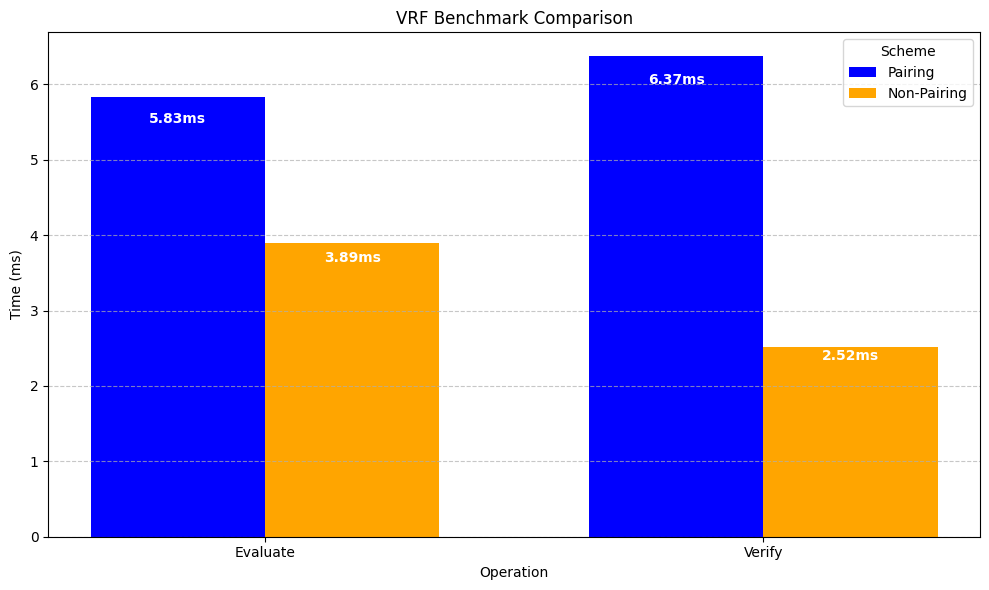
\includegraphics[width=0.75\linewidth]{figures/vrf-benchmark.png}
    \caption{VRF Benchmark}
    \label{fig:vrf-benchmark}
\end{figure}








% \subsection{CRBN Instantiation In Identity System}

% The Credential Relationship Binding Nullifier (CRBN) extends the Multi-Issuer Multi-Credential Anonymous Credential (MIMC-ABC) system from Chapter 3 to support a hierarchical structure with sybil resistance. We define two credential types: a \emph{Master Credential} containing a secret key $\k$, and \emph{Context Credentials} with context identifiers $\ctx$. A nullifier $\nul = g^{1/(\k + \ctx)} \in \G$ binds each Context Credential to the Master Credential, ensuring uniqueness per context while preserving privacy via zero-knowledge proofs.

% We modify MIMC-ABC’s algorithms as follows, reusing its position-binding Pedersen commitments and $\Sigma$-protocols. Let $\mathsf{pp}$ include $\G$, $p$, $g$, and commitment generators $(g_1, g_2, g_3, g_4, g)$, where $\ell = 4$ supports attributes $[\id, \ctx, \exp, \k]$ (extensible to more).

% \begin{itemize}
%     \item \textbf{Master Credential Issuance}:
%     \begin{itemize}
%         \item \emph{User}: Samples $\k \sample \Z_p$ and $\usk_m \sample \Z_p$. Computes commitment $\cmm = g_1^\id g_2^{\ctx_m} g_3^{\exp_m} g_4^\k g^{\usk_m}$, where $\ctx_m = \mathcal{H}(\text{"master"})$ and $\exp_m$ is the expiration. Runs $\mathsf{Obtain}(\attrs_m = [\id, \ctx_m, \exp_m, \k], \{\mathsf{opk}_j\}, \usk_m)$ with issuer $j_m$, proving $\cmm$’s opening via $\pircom$ (Section 2.4.3).
%         \item \emph{Issuer $j_m$}: Verifies the proof, signs $\sigma_m = \mathsf{RS.Sign}(\cmm, \mathsf{osk}_{j_m})$, and returns $\credm = (\sigma_m, \cmm)$ via $\mathsf{Issue}$.
%     \end{itemize}

%     \item \textbf{Context Credential Issuance}:
%     \begin{itemize}
%         \item \emph{User}: For context $\ctx_c$ (e.g., $\mathcal{H}(\text{"DMV"})$), samples $\usk_c \sample \Z_p$. Computes $\cmc = g_1^\id g_2^{\ctx_c} g_3^{\exp_c} g^{\usk_c}$ (no $\k$ here, as it’s from $\credm$). Runs $\mathsf{Obtain}(\attrs_c = [\id, \ctx_c, \exp_c, 0], \{\mathsf{opk}_j\}, \usk_c)$ with issuer $j_c$, proving $\cmc$’s opening and that position 4 is 0.
%         \item \emph{Issuer $j_c$}: Verifies the proof, optionally checks a nullifier registry (see below), signs $\sigma_c = \mathsf{RS.Sign}(\cmc, \mathsf{osk}_{j_c})$, and returns $\credc = (\sigma_c, \cmc)$.
%     \end{itemize}

%     \item \textbf{Nullifier Generation}: Given $\credm$ with $\k$ and $\credc$ with $\ctx_c$, compute:
%     \[
%     \nul = g^{1/(\k + \ctx_c)} \in \G
%     \]
%     where $\k + \ctx_c$ is computed in $\Z_p$, and the inverse $1/(\k + \ctx_c)$ exists with overwhelming probability (as $p$ is prime).

%     \item \textbf{Presentation and Verification}:
%     \begin{itemize}
%         \item \emph{User}: Inputs $\credm$, $\credc$, $\usk_m$, $\usk_c$, and a predicate $\phi$ (e.g., $\ctx_c = \text{"DMV"} \land \exp_c > \text{today}$). Rerandomizes $\credm$ to $(\sigma_m', \cmm')$ and $\credc$ to $(\sigma_c', \cmc')$ using $\Delta_{r_m}, \Delta_{r_c}$ (Section 3.3). Computes $\nul = g^{1/(\k + \ctx_c)}$ and proves:
%         \[
%         \mathcal{R}_{\mathsf{vrf}} = \zkpok \left\{ 
%         (\cmm', \cmc', \nul), (\id, \ctx_m, \exp_m, \k, \usk_m', \ctx_c, \exp_c, \usk_c') 
%         \middle|
%         \begin{array}{l}
%         \cmm' = g_1^\id g_2^{\ctx_m} g_3^{\exp_m} g_4^\k g^{\usk_m'} \land \ctx_m = \mathcal{H}(\text{"master"}) \land \\
%         \mathsf{RS.Ver}(\sigma_m', \cmm', \mathsf{opk}_{j_m}) = 1 \land \\
%         \cmc' = g_1^\id g_2^{\ctx_c} g_3^{\exp_c} g^{\usk_c'} \land \\
%         \mathsf{RS.Ver}(\sigma_c', \cmc', \mathsf{opk}_{j_c}) = 1 \land \\
%         \nul = g^{1/(\k + \ctx_c)} \land \phi(\ctx_c, \exp_c) = 1
%         \end{array} 
%         \right\}
%         \]
%         where $\usk_m' = \usk_m + \Delta_{r_m}$, $\usk_c' = \usk_c + \Delta_{r_c}$. The proof uses the $\Sigma$-protocol from Section 4.x (to be detailed).
%         \item \emph{Verifier}: Checks $\pi$, $\sigma_m'$, $\sigma_c'$, and $\nul$ against $\mathsf{opk}_{j_m}$, $\mathsf{opk}_{j_c}$. Optionally queries a nullifier registry to ensure $\nul$ is unused for $\ctx_c$.
%     \end{itemize}
% \end{itemize}

% \textbf{Note on Revocation}: If $\credm$ is revoked (e.g., via a public revocation list for $\cmm$ or $\k$), verifiers can reject proofs involving $\nul$, as $\k$’s validity underpins $\mathcal{R}_{\mathsf{vrf}}$. Details are deferred to Section 4.y.

% \textbf{Note on Sybil Resistance}: Issuers or verifiers may maintain a context-specific nullifier registry. During issuance, users prove $\nul$’s correctness in zero-knowledge; issuers reject duplicates. Alternatively, verifiers check $\nul$’s uniqueness during presentation, balancing privacy and accountability (see Section 4.z).

% This construction leverages MIMC-ABC’s efficient $\Sigma$-protocols and avoids pairings, using only standard group operations in $\G$. The nullifier $\nul$ enforces hierarchical binding and sybil resistance, computed deterministically from $\k$ and $\ctx_c$.





\begin{table}
\begin{center}
\caption{Comparison of our construction over previous work.}
\label{tab:comparison-chap4}
\begin{tabular}{l|ccccc}
Features    									& 
Sybil Resist.  & 
Hierarchy & 
Private & 
Pairing-Free & 
Predicate Proofs \\
\hline
CanDID \cite{maram2021candid}     				&
\ding{51}     & 
\ding{51} 	& 
\ding{55}  &  
-     & 
\ding{55}		\\
SyRA \cite{crites_syra_2024}     				& 
\ding{51}    	& 
\ding{51}     & 
\ding{51}  &  
\ding{51}     & 
\ding{55}		\\
S3ID \cite{rabaninejad_attribute-based_2024}  & 
\ding{51}     & 
\ding{51}    	& 
\ding{55}  &  
\ding{55}     & 
\ding{55}		\\
UTT               & 
\ding{51}     & 
\ding{51}    	& 
\ding{51}  &  
\ding{55}     & 
\ding{51}		\\
Chap3             & 
\ding{55}     & 
\ding{55}    	& 
\ding{51}  &  
\ding{55}     & 
\ding{51}		\\
Ours  										& 
\ding{51}     & 
\ding{51}    	& 
\ding{51}  &  
\ding{51}     & 
\ding{51}		\\
\end{tabular}
\end{center}
\vspace{1em}
\footnotetext[1]{Predicate Proofs allow users to prove statements about their credentials privately}
\footnotetext[2]{Efficient Token refers to optimization of token verification}
\end{table}